\documentclass{standalone}
\usepackage{tikz}
\usepackage{xcolor}

\begin{document}
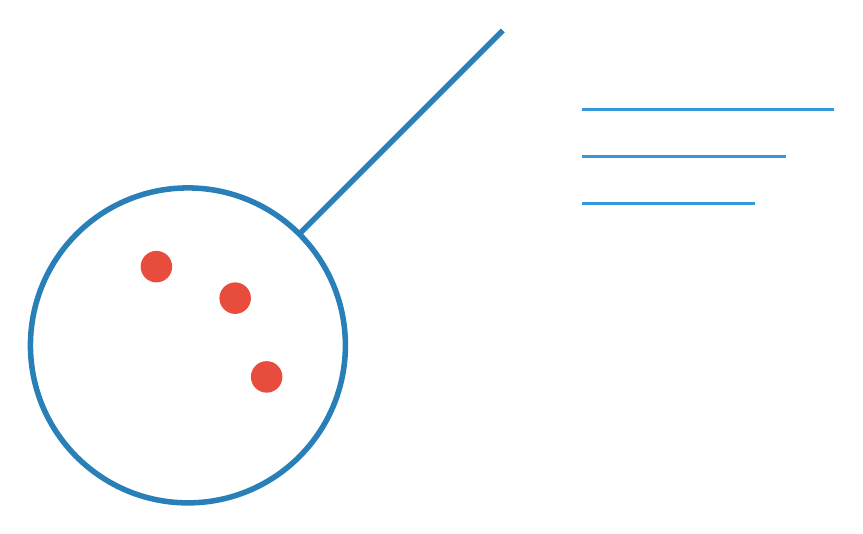
\begin{tikzpicture}[scale=2]
    % Define colors
    \definecolor{primary}{RGB}{41, 128, 185}
    \definecolor{secondary}{RGB}{52, 152, 219}
    \definecolor{accent}{RGB}{231, 76, 60}
    
    % Draw magnifying glass
    \draw[line width=2pt, primary] (0,0) circle (1);
    \draw[line width=2pt, primary] (45:1) -- (2,2);
    
    % Draw search results
    \foreach \i in {0,1,2} {
        \draw[line width=1pt, secondary] (2.5+\i*0.3, 1.5) -- (3.5+\i*0.3, 1.5);
        \draw[line width=1pt, secondary] (2.5+\i*0.3, 1.2) -- (3.2+\i*0.3, 1.2);
        \draw[line width=1pt, secondary] (2.5+\i*0.3, 0.9) -- (3.0+\i*0.3, 0.9);
    }
    
    % Add accent elements
    \fill[accent] (0.3,0.3) circle (0.1);
    \fill[accent] (-0.2,0.5) circle (0.1);
    \fill[accent] (0.5,-0.2) circle (0.1);
\end{tikzpicture}
\end{document} 